\section{Experimental evaluations}

\subsection{Experimental setup}

We perform our experiments on odroidxue devices which are a small mobile like devices with Ubuntu 14.04 running on them. These devices have 19 speed settings with all being available for its 4 big cores and 13 for four LITTLE cores. Thus in total we have 128 user accessible configurations. Each configuration has a different performance and power. We use 20 different benchmarks from five different suites including PARSEC
(\texttt{blackscholes},\texttt{facesim}, \texttt{x264} ) \cite{parsec}, 
Minebench
(\texttt{Kmeans},  
\texttt{non fuzzy kmeans \\* (Kmeansnf)}) \cite{minebench}, 
Seec
(\texttt{dijkstra}) \cite{seec}, 
Parmibench
(\texttt{ferret}) \cite{parmibench}, and Rodinia
(\texttt{backprop},\texttt{cfd}, \texttt{nn}, \texttt{lud}, \\* 
\texttt{backprop}, \texttt{bfs}) \cite{rodinia}.  
We also use a
partial differential equation solver (\texttt{jacobi}) and a memory intensive benchmark pair (\texttt{stream}) and (\texttt{stream\_threads}) \cite{stream}. Our benchmarks vary from compute-bound applications to memory bound workloads and also workloads that are a combination of both as shown in \figref{application_variety}.
Our applications have been instrumented with heartbeat library to report heartbeats/second as a measure of performance \cite{poet}.

\subsection{Evaluation metrics}
We use LEO to estimate the performance and power for our applications. The accuracy of LEO for learning is measured as,
\begin{equation}
\label{eq:accuracy}
accuracy(\hat{\y},\y) = max\left(1 - \frac{\| \hat{\y}-\y \|^2_2 }{\| \y - \bar{\y}\|^2_2},0\right).
\end{equation}

where $\hat{\y}$ represents the predicted performance and power values and $\y$ is the true value of the power and performance.

Our \SYSTEM{} uses the model for power and performance and its controller actively uses this knowledge to meet the performance target. A performance target can be thought of as a quality of service expectation for the given application. We run our applications from 10\% to 90\% performance targets and observe how our \SYSTEM{} performs under each constraint. we quantify how well the applications are meeting the target by using the commonly used metric called MAPE. Suppose the application is supposed to finish $n$ jobs while maintaining a speed of $S_r$, then MAPE is as shown below,

\begin{equation}
MAPE = 100\% \cdot \frac{1}{n} \sum\limits_{i=1}^{n} max \left( \frac{S_{r} - s_m(i)}{S_r},0 \right)
\end{equation}

where $S_{r}$ is the performance target and $s_m(i)$ is the performance observed for $i$th job.

\begin{figure*}
\centering
%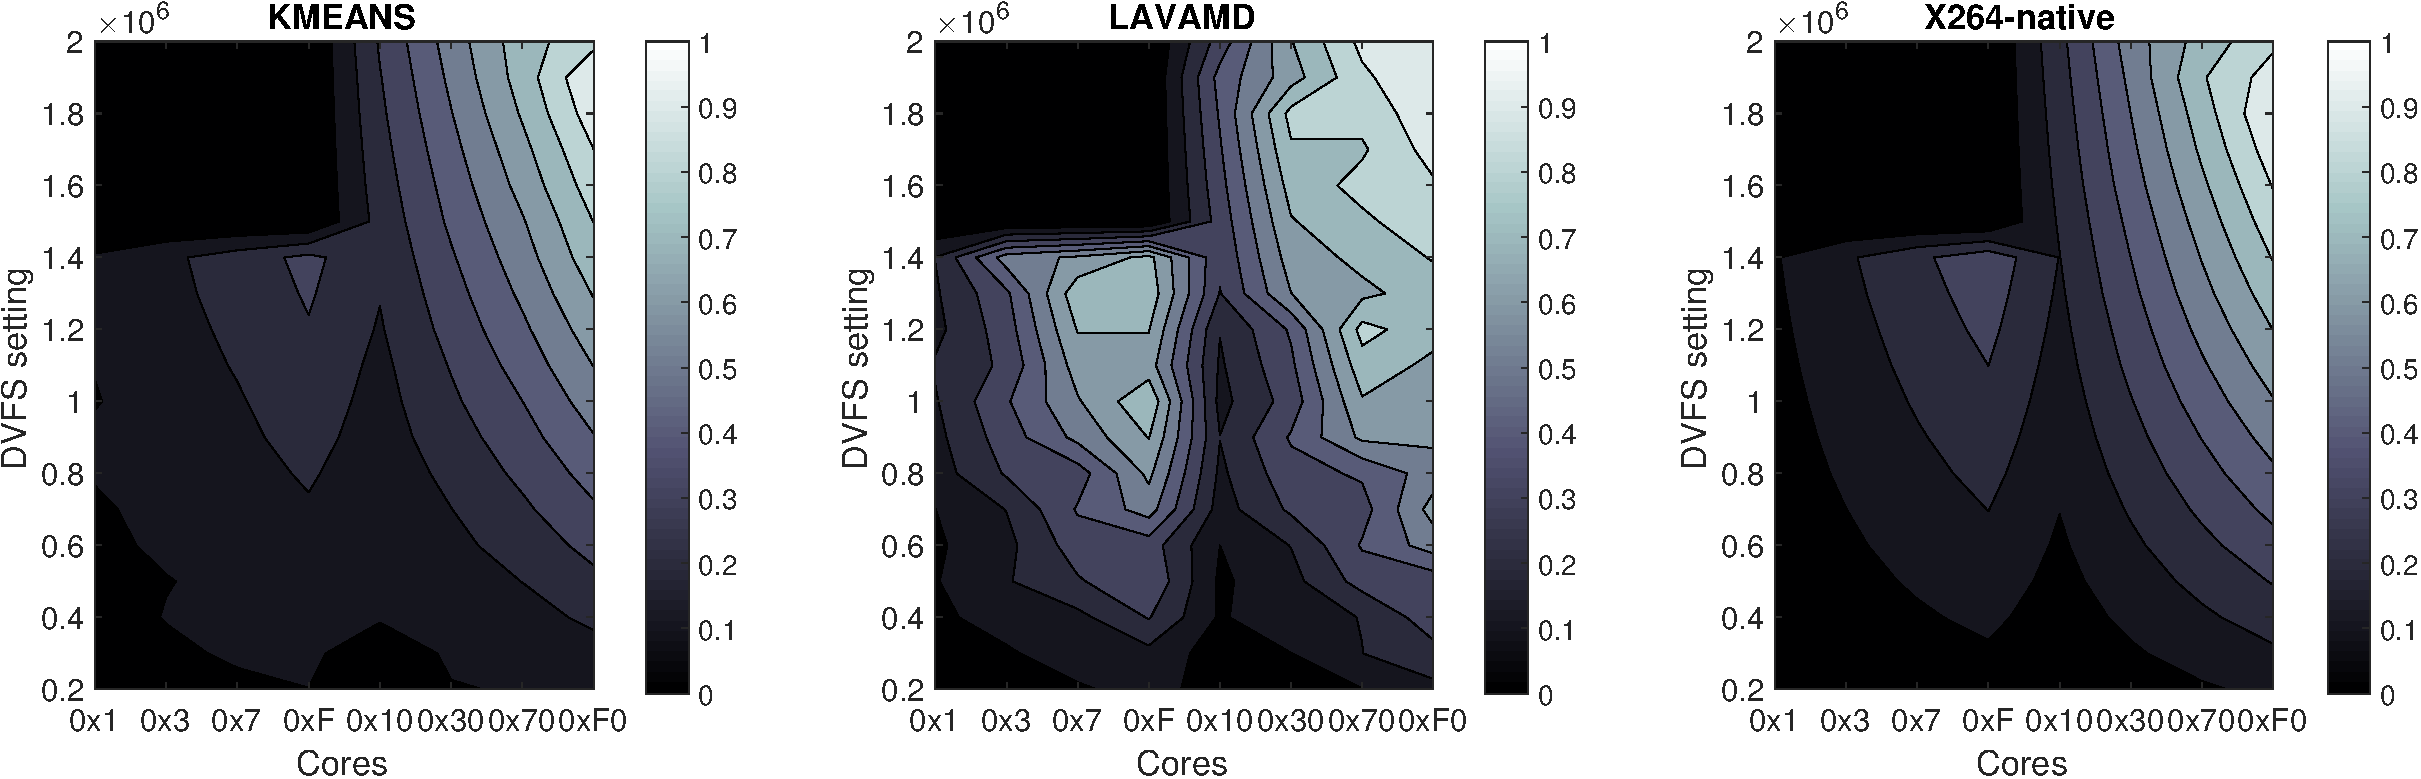
\includegraphics[width=\paperwidth,scale=0.5]{figures/performance-contour3.pdf}
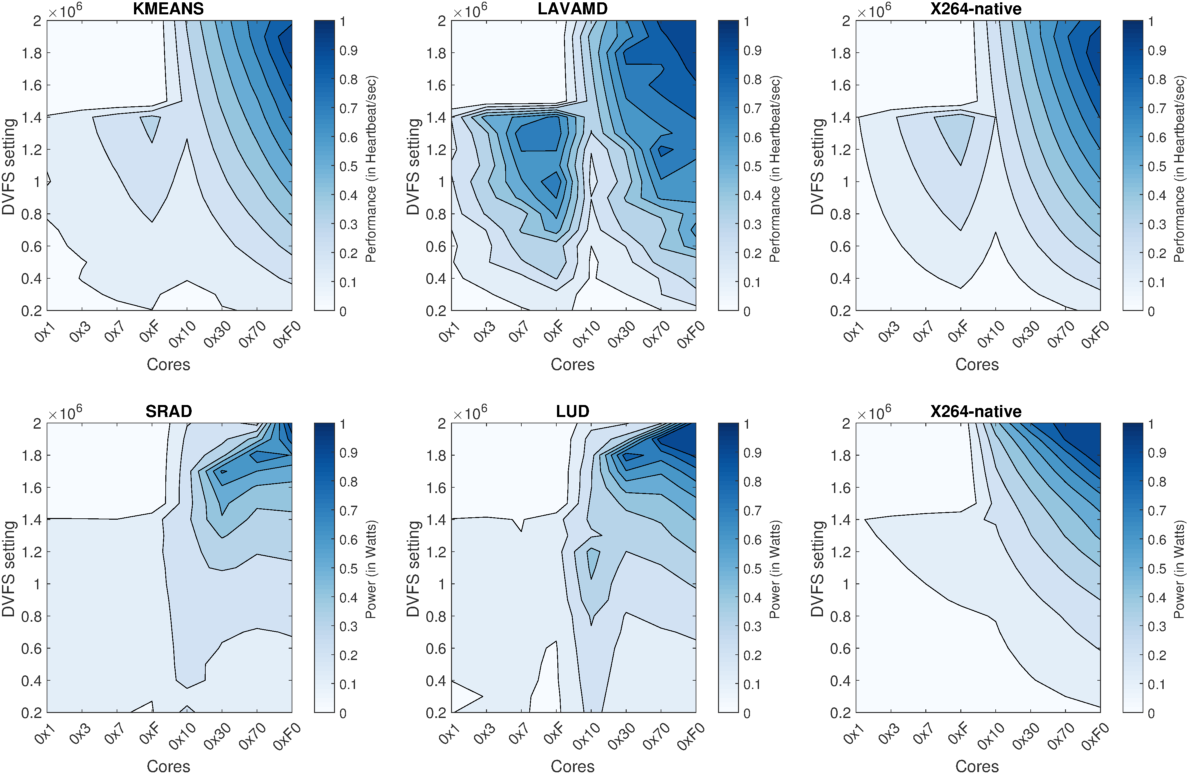
\includegraphics[scale=0.4]{figures/sample-contour3.png}

\caption{Contour.}
  \label{fig:contour}
\end{figure*}
\subsection{Points of comparison}
We first compare the prediction accuracy for our machine learning model LEO to the following algorithms.

\begin{enumerate}
\item \textit{Online} -- This strategy carries out polynomial
  multivariate regression on the observed dataset using configuration
  values (the number of cores and speed-settings) as
  predictors, and estimates the rest of the data-points based the same
  model. The learnt model is then sent to the controller. Note that the process of collecting samples for estimation might be very expensive and this model requires a minimum number of samples to start with. This method uses only the observations and
  not the prior data.
\item \textit{Offline} -- This is our zero-sample policy. This method takes the mean over the rest of the applications to estimate the power and performance of the given application and uses these predictions for the controller.
  This strategy only uses prior information and does not update the model
  based on runtime observations.
\end{enumerate}
We later compare \SYSTEM{} to the baselines constructed with a combination of different learning models and a state-of-art controller based on \emph{Pace-to-idle(P2I)} heuristic which has been proven to be a better heuristic than \emph{Race-to-idle} \cite{RACINGPACING}. 
\begin{enumerate}
\item \textit{Online-P2I} -- We use the \textit{Online} learning model in combination with  \emph{Pace-to-idle(P2I)} heuristic.
\item \textit{Offline-P2I} -- We use the \textit{Offline} learning model in combination with  \emph{Pace-to-idle(P2I)} heuristic.
\item \textit{LEO-P2I} -- We use the \textit{LEO} learning model in combination with  \emph{Pace-to-idle(P2I)} heuristic.
\item \textit{POET} -- We use the \textit{offline} learning model in combination with  \emph{POET} controller. 
\end{enumerate}

\subsection{Power and performance estimation}

We used LEO as described in \secref{sec:framework:HBM} to estimate the power and performance for the applications using only 10 out of 128 observations. The true performance and power frontiers for the applications are very unusual for some applications with multiple local minima across the configuration space as shown in \figref{fig:contour}. Therefore, line-search based techniques for  resources allocation (cores/clockspeed) to directly improve or reduce performance isn't optimal since we might end up in a local minima. In  \figref{fig:contour}, we can see that 
the performance plot for the applications \texttt{Kmeans},\texttt{lavamd} and \texttt{X264} 
against the clockspeed and cores is non-convex and contains at least 2 local minima corresponding to big and LITTLE cores. 
Similarly, we have power plot for 3 applications and the surface seems very non-smooth. The non-smoothness of the surface is the reason why parametric models over these curves do not perform well and technique, which is non-parametric hence is not affected by the shape of the curve, but rather depends on the application behavior being similar to at least one other application seems to work pretty well.

Our results are summarized in \figref{fig:accuracy}. LEO is 13.4\% better than online and 19.1\% better than offline in terms of performance estimation and LEO is 3.7\% better than online and 1.5\% better than offline in terms of power estimation, on average over all the benchmarks. %Infact, LEO uniformly performs well for all applications with the worst accuracy being YY as compared to offline and online algorithm.


\begin{figure*}[t]
  \begin{tikzpicture}
\definecolor{s1}{RGB}{228, 26, 28}
\definecolor{s2}{RGB}{55, 126, 184}
\definecolor{s3}{RGB}{77, 175, 74}
\definecolor{s4}{RGB}{152, 78, 163}
\definecolor{s5}{RGB}{255, 127, 0}

\begin{groupplot}[
    group style={
        group name=plots,
        group size=1 by 1,
        xlabels at=edge top,
        xticklabels at=edge top,
        vertical sep=5pt
    },
axis x line* = top,
xlabel near ticks,
major x tick style = transparent,
height=3cm,
width=0.88\textwidth,
xmin=0,
xmax=9,
enlargelimits=false,
tick align = outside,
tick style={white},
ylabel style={align=center},
ytick=\empty,
xtick=\empty,
xticklabels={},
yticklabels={},
ymin=0,
ymax=1,
]
\nextgroupplot[ylabel={},
y label style={rotate=270},
ylabel shift={12mm},
]
\addplot[thick,solid, color=black] coordinates {(0,1) (22,1)};

\nextgroupplot[
ylabel shift={12mm},
y label style={rotate=270},
ylabel={$\mathsf{30\%}$},
]
\addplot[thick,solid, color=black] coordinates {(0,1) (22,1)};

\nextgroupplot[
ylabel shift={12mm},
y label style={rotate=270},
ylabel={$\mathsf{50\%}$},
]
\addplot[thick,solid, color=black] coordinates {(0,1) (22,1)};


\nextgroupplot[
ylabel shift={12mm},
ylabel={$\mathsf{70\%}$},
y label style={rotate=270},
]
\addplot[thick,solid, color=black] coordinates {(0,1) (22,1)};

\nextgroupplot[
ylabel shift={12mm},
ylabel={$\mathsf{90\%}$},
y label style={rotate=270},
]
\addplot[thick,solid, color=black] coordinates {(0,1) (22,1)};

\end{groupplot}

\begin{groupplot}[
    group style={
        group name=plots,
        group size=1 by 2,
        xlabels at=edge bottom,
        xticklabels at=edge bottom,
        vertical sep=5pt
    },
axis x line* = bottom,
xlabel near ticks,
major x tick style = transparent,
xlabel={},
height=3cm,
width=0.88\textwidth,
xmin=0,
xmax=22,
enlargelimits=false,
tick align = outside,
tick style={white},
ylabel style={align=center},
ytick=\empty,
ymin=0,
ymax=1.1,
ytick={0,0.3,0.6,0.9},
yticklabels={,0.3,0.6,0.9},
legend cell align=left, 
legend style={ column sep=1ex },
ymajorgrids,
grid style={dashed},
]


\nextgroupplot[ybar=\pgflinewidth,
bar width=2.0pt,
legend entries = {{$\mathsf{Online}$},{$\mathsf{Offline}$},{$\mathsf{LEO}$}},
legend style={draw=none,legend columns=3,at={(.5,1.7)},anchor=north},
ylabel={\footnotesize Accuracy\\ (Performance)}, 
ylabel shift={0mm},
]
\addplot table[x index=0,y index=5, col sep=space] {img/image_text/accuracy.txt};
\addplot table[x index=0,y index=7, col sep=space] {img/image_text/accuracy.txt};
\addplot table[x index=0,y index=3, col sep=space] {img/image_text/accuracy.txt};

\nextgroupplot[ybar=\pgflinewidth,
bar width=2.0pt,
ylabel={\footnotesize Accuracy\\ (Power)}, 
ylabel shift={0mm},
xticklabel shift={0pt},
x tick label style={rotate=35, anchor=east},
xtick={1,2,3,4,5,6,7,8,9,10,11,12,13,14,15,16,17,18,19,20,21,22},
xticklabels={
{\scriptsize $\mathsf{backprop}$},
{\scriptsize $\mathsf{bfs}$},
{\scriptsize $\mathsf{blackscholes}$},
{\scriptsize $\mathsf{bodytrack}$},
{\scriptsize $\mathsf{facesim}$},
{\scriptsize $\mathsf{ferret}$},
{\scriptsize $\mathsf{heartwall}$},
{\scriptsize $\mathsf{hotspot}$},
{\scriptsize $\mathsf{jacobi}$},
{\scriptsize $\mathsf{kmeans}$},
{\scriptsize $\mathsf{kmeansnf}$},
{\scriptsize $\mathsf{lavamd}$},
{\scriptsize $\mathsf{leukocyte}$},
{\scriptsize $\mathsf{lud}$},
{\scriptsize $\mathsf{nw}$},
{\scriptsize $\mathsf{sha}$},
{\scriptsize $\mathsf{srad}$},
{\scriptsize $\mathsf{stream_threads}$},
{\scriptsize $\mathsf{x264-ducks}$},
{\scriptsize $\mathsf{x264-native}$},
{\scriptsize $\mathsf{\mathbf{Average}}$}},
]
\addplot table[x index=0,y index=4, col sep=space] {img/image_text/accuracy.txt};
\addplot table[x index=0,y index=6, col sep=space] {img/image_text/accuracy.txt};
\addplot table[x index=0,y index=2, col sep=space] {img/image_text/accuracy.txt};

\end{groupplot}
\end{tikzpicture}
   \vskip -1em
  \caption{Accuracy performance}
  \label{fig:accuracy}
\end{figure*}

\subsubsection{Sensitivity to the measured samples}
Now we look into some results on how sensitive LEO is to varying the number of samples for estimation. Odroid devices are quite small and sampling overhead can be quite expensive hence it is important that our methods do not require huge number of samples. In \figref{fig:sensitivity} we observe that when no samples are available LEO performs as well as Offline approach and as it gets more samples the accuracy uniformly improves and reaches greater than 90\% with around 20 samples. On the other hand, the online approach needs at least 9 samples so that the design matrix for the polynomial regression has more samples than variables. As we get more samples the accuracy for online model improves but still does not meet the accuracy that LEO can achieve for same number of samples.

\begin{figure}[t]
  \begin{tikzpicture}
\begin{centering}

\definecolor{s1}{RGB}{228, 26, 28}
\definecolor{s2}{RGB}{55, 126, 184}
\definecolor{s3}{RGB}{77, 175, 74}
\definecolor{s4}{RGB}{152, 78, 163}
\definecolor{s5}{RGB}{255, 127, 0}

\begin{groupplot}[
    group style={
        group name=plots,
        group size=1 by 2,
        xlabels at=edge bottom,
        xticklabels at=edge bottom,
        vertical sep=5pt
    },
height=3.5cm,
width=0.95\columnwidth,
xmajorgrids,
ymajorgrids,
grid style={dashed},
xmin=0,
xmax=100,
yticklabel pos=left,
enlargelimits=false,
tick align = outside,
tick style={white},
xticklabel shift={-5pt},
yticklabel shift={-5pt},
ylabel shift={-2pt},
ylabel style={align=center},
unbounded coords=jump,
]

\nextgroupplot[ylabel={\footnotesize Accuracy\\(Performance)}, % Performance
xtick={0,20,40,60,80,100},
ytick={0.0,0.3,0.6,0.9,1.0},
yticklabels={,0.3,0.6,0.9,1.0},
yticklabel style={font=\footnotesize},
ymin=0,
ymax=1,
legend entries={{$\mathsf{Online}$},{$\mathsf{\SYSTEM{}}$}},
legend style={draw=none,at={(0.5,1.4)},anchor=north,legend columns=4,line width=5pt},
]
%\addplot[thick, solid, color=s3] table[x index=0,y index=1,col sep=tab] {img/old/x264-phases-clover-dvfs.txt};

\addplot[thick, solid, color=s4] table[x index=0,y index=3,col sep=tab] {img/sample_accuracy.txt};
\addplot[thick, solid, color=s3] table[x index=0,y index=1,col sep=tab] {img/sample_accuracy.txt};
%\addplot[thick, solid, black] coordinates {(0, 1) (4500, 1)};
%\addplot[thick, dashed, black] coordinates {(1500,0) (1500, 2)};
%\addplot[thick, dashed, black] coordinates {(3000,0) (3000, 2)};


\nextgroupplot[ylabel={\footnotesize Accuracy\\ (Power)}, % Power
ytick={0.0,0.3,0.6,0.9,1.0},
yticklabels={,0.3,0.6,0.9,1.0},
yticklabel style={font=\footnotesize},
ymin=0,
ymax=1,
xlabel={\footnotesize \% Samples for training},
xlabel near ticks,
xtick={0,20,40,60,80,100},
xticklabels={0,20,40,60,80,100},
xticklabel style={font=\footnotesize},
]

\addplot[thick, solid, color=s4] table[x index=0,y index=4,col sep=tab] {img/sample_accuracy.txt};
\addplot[thick, solid, color=s3] table[x index=0,y index=2,col sep=tab] {img/sample_accuracy.txt};
%\addplot[thick, dashed, black] coordinates {(1500,0) (1500, 250)};
%\addplot[thick, dashed, black] coordinates {(3000,0) (3000, 250)};

\end{groupplot}
\end{centering}

\end{tikzpicture}

   \vskip -1em
  \caption{Multi Applications Energy}
  \label{fig:sensitivity}
\end{figure}

\subsection{\SYSTEM{}}
\subsubsection{Single application}
In this section, we demonstrate how \SYSTEM{} performs in in terms of energy consumption and MAPE throughout the runtime of an application for different performance targets. The performance targets have been set up to measure the capabilities of \SYSTEM{} under different scenarios. 10\% performance target corresponds to low performance target and a good static strategy might be to choose lower configurations to conserve energy, on the other hand 90\% performance target would mean the application requires to run in fast, hence we could choose highest configurations since MAPE is generally minimized at the highest configurations. The interesting performance targets are around 30\%-70\% where we don't have obvious choices for configuration settings to either save energy or minimize MAPE. We find that \SYSTEM{} has lower MAPE and energy consumption than the baseline algorithms. \TODO{some more specific example}. As shown in \figref{fig:single-perf} and \figref{fig:single-energy}, \SYSTEM{} uniformly has the smaller MAPE

\begin{figure*}[t]
  \begin{tikzpicture}
\definecolor{s1}{RGB}{228, 26, 28}
\definecolor{s2}{RGB}{55, 126, 184}
\definecolor{s3}{RGB}{77, 175, 74}
\definecolor{s4}{RGB}{152, 78, 163}
\definecolor{s5}{RGB}{255, 127, 0}

\begin{groupplot}[
    group style={
        group name=plots,
        group size=1 by 5,
        xlabels at=edge top,
        xticklabels at=edge top,
        vertical sep=5pt
    },
axis x line* = top,
xlabel near ticks,
major x tick style = transparent,
height=2.5cm,
width=0.88\textwidth,
xmin=0,
xmax=9,
enlargelimits=false,
tick align = outside,
tick style={white},
ylabel style={align=center},
ytick=\empty,
xtick=\empty,
xticklabels={},
yticklabels={},
ymin=0,
ymax=1,
]
\nextgroupplot[ylabel={$\mathsf{10\%}$},
y label style={rotate=270},
ylabel shift={12mm},
]
\addplot[thick,solid, color=black] coordinates {(0,1) (22,1)};

\nextgroupplot[
ylabel shift={12mm},
y label style={rotate=270},
ylabel={$\mathsf{30\%}$},
]
\addplot[thick,solid, color=black] coordinates {(0,1) (22,1)};

\nextgroupplot[
ylabel shift={12mm},
y label style={rotate=270},
ylabel={$\mathsf{50\%}$},
]
\addplot[thick,solid, color=black] coordinates {(0,1) (22,1)};


\nextgroupplot[
ylabel shift={12mm},
ylabel={$\mathsf{70\%}$},
y label style={rotate=270},
]
\addplot[thick,solid, color=black] coordinates {(0,1) (22,1)};

\nextgroupplot[
ylabel shift={12mm},
ylabel={$\mathsf{90\%}$},
y label style={rotate=270},
]
\addplot[thick,solid, color=black] coordinates {(0,1) (22,1)};

\end{groupplot}

\begin{groupplot}[
    group style={
        group name=plots,
        group size=1 by 5,
        xlabels at=edge bottom,
        xticklabels at=edge bottom,
        vertical sep=5pt
    },
axis x line* = bottom,
xlabel near ticks,
major x tick style = transparent,
xlabel={},
height=2.5cm,
width=0.88\textwidth,
xmin=0,
xmax=22,
enlargelimits=false,
tick align = outside,
tick style={white},
ylabel style={align=center},
ytick=\empty,
ymin=0,
ymax=30,
ytick={0,5,10,15,20},
yticklabels={,5,10,15,20},
legend cell align=left, 
legend style={ column sep=1ex },
ymajorgrids,
grid style={dashed},
]

\nextgroupplot[ybar=\pgflinewidth,
bar width=2.0pt,
legend entries = {{$\mathsf{Online-P2I}$},{$\mathsf{Offline-P2I}$},{$\mathsf{LEO-P2I}$},{$\mathsf{POET}$},{$\mathsf{\SYSTEM{}}$}},
legend style={draw=none,legend columns=5,at={(.5,1.7)},anchor=north},
ylabel shift={0mm},
ymin=0,
ymax=6,
ytick={0.0,2.0,4.0,6.0},
yticklabels={,2.0,4.0,6.0},
]
\addplot table[x index=0,y index=3, col sep=space] {img/image_text/dyn-mape-0.1.txt};
\addplot table[x index=0,y index=4, col sep=space] {img/image_text/dyn-mape-0.1.txt};
\addplot table[x index=0,y index=5, col sep=space] {img/image_text/dyn-mape-0.1.txt};
\addplot table[x index=0,y index=6, col sep=space] {img/image_text/dyn-mape-0.1.txt};
\addplot table[x index=0,y index=7, col sep=space] {img/image_text/dyn-mape-0.1.txt};

\nextgroupplot[ybar=\pgflinewidth,
ylabel shift={0mm},
bar width=2.0pt,
ymin=0,
ymax=20,
ytick={0.0,5.0,10.0,15.0,20.0},
yticklabels={,5.0,10.0,15.0},
]
\addplot table[x index=0,y index=3, col sep=space] {img/image_text/dyn-mape-0.3.txt};
\addplot table[x index=0,y index=4, col sep=space] {img/image_text/dyn-mape-0.3.txt};
\addplot table[x index=0,y index=5, col sep=space] {img/image_text/dyn-mape-0.3.txt};
\addplot table[x index=0,y index=6, col sep=space] {img/image_text/dyn-mape-0.3.txt};
\addplot table[x index=0,y index=7, col sep=space] {img/image_text/dyn-mape-0.3.txt};

\nextgroupplot[ybar=\pgflinewidth,
ylabel={\footnotesize MAPE},
ylabel shift={0mm},
bar width=2.0pt,
ymin=0,
ymax=30,
ytick={0.0,10.0,20.0,30.0},
yticklabels={,10.0,20.0,30.0},
]
\addplot table[x index=0,y index=3, col sep=space] {img/image_text/dyn-mape-0.5.txt};
\addplot table[x index=0,y index=4, col sep=space] {img/image_text/dyn-mape-0.5.txt};
\addplot table[x index=0,y index=5, col sep=space] {img/image_text/dyn-mape-0.5.txt};
\addplot table[x index=0,y index=6, col sep=space] {img/image_text/dyn-mape-0.5.txt};
\addplot table[x index=0,y index=7, col sep=space] {img/image_text/dyn-mape-0.5.txt};

\nextgroupplot[ybar=\pgflinewidth,
ylabel shift={0mm},
bar width=2.0pt,
ymin=0,
ymax=30,
ytick={0.0,10.0,20.0,30.0},
yticklabels={,10.0,20.0,30.0},
]
\addplot table[x index=0,y index=3, col sep=space] {img/image_text/dyn-mape-0.7.txt};
\addplot table[x index=0,y index=4, col sep=space] {img/image_text/dyn-mape-0.7.txt};
\addplot table[x index=0,y index=5, col sep=space] {img/image_text/dyn-mape-0.7.txt};
\addplot table[x index=0,y index=6, col sep=space] {img/image_text/dyn-mape-0.7.txt};
\addplot table[x index=0,y index=7, col sep=space] {img/image_text/dyn-mape-0.7.txt};

\nextgroupplot[ybar=\pgflinewidth,
bar width=2.0pt,
ylabel shift={0mm},
xticklabel shift={0pt},
ymin=0,
ymax=30,
ytick={0.0,10.0,20.0,30.0},
yticklabels={,10.0,20.0,30.0},
x tick label style={rotate=35, anchor=east},
xtick={1,2,3,4,5,6,7,8,9,10,11,12,13,14,15,16,17,18,19,20,21,22},
xticklabels={
{\scriptsize $\mathsf{backprop}$},
{\scriptsize $\mathsf{bfs}$},
{\scriptsize $\mathsf{blackscholes}$},
{\scriptsize $\mathsf{bodytrack}$},
{\scriptsize $\mathsf{facesim}$},
{\scriptsize $\mathsf{ferret}$},
{\scriptsize $\mathsf{heartwall}$},
{\scriptsize $\mathsf{hotspot}$},
{\scriptsize $\mathsf{jacobi}$},
{\scriptsize $\mathsf{kmeans}$},
{\scriptsize $\mathsf{kmeansnf}$},
{\scriptsize $\mathsf{lavamd}$},
{\scriptsize $\mathsf{leukocyte}$},
{\scriptsize $\mathsf{lud}$},
{\scriptsize $\mathsf{nw}$},
{\scriptsize $\mathsf{sha}$},
{\scriptsize $\mathsf{srad}$},
{\scriptsize $\mathsf{stream_threads}$},
{\scriptsize $\mathsf{x264-ducks}$},
{\scriptsize $\mathsf{x264-native}$},
{\scriptsize $\mathsf{\mathbf{Average}}$}},
]
\addplot table[x index=0,y index=3, col sep=space] {img/image_text/dyn-mape-0.9.txt};
\addplot table[x index=0,y index=4, col sep=space] {img/image_text/dyn-mape-0.9.txt};
\addplot table[x index=0,y index=5, col sep=space] {img/image_text/dyn-mape-0.9.txt};
\addplot table[x index=0,y index=6, col sep=space] {img/image_text/dyn-mape-0.9.txt};
\addplot table[x index=0,y index=7, col sep=space] {img/image_text/dyn-mape-0.9.txt};

\end{groupplot}
\end{tikzpicture}
   \vskip -1em
  \caption{Single Applications MAPE}
  \label{fig:single-perf}
\end{figure*}

\begin{figure*}[t]
  \begin{tikzpicture}
\definecolor{s1}{RGB}{228, 26, 28}
\definecolor{s2}{RGB}{55, 126, 184}
\definecolor{s3}{RGB}{77, 175, 74}
\definecolor{s4}{RGB}{152, 78, 163}
\definecolor{s5}{RGB}{255, 127, 0}

\begin{groupplot}[
    group style={
        group name=plots,
        group size=1 by 5,
        xlabels at=edge top,
        xticklabels at=edge top,
        vertical sep=5pt
    },
axis x line* = top,
xlabel near ticks,
major x tick style = transparent,
height=2.5cm,
width=0.88\textwidth,
xmin=0,
xmax=9,
enlargelimits=false,
tick align = outside,
tick style={white},
ylabel style={align=center},
ytick=\empty,
xtick=\empty,
xticklabels={},
yticklabels={},
ymin=0,
ymax=1,
]
\nextgroupplot[ylabel={$\mathsf{10\%}$},
y label style={rotate=270},
ylabel shift={12mm},
]
\addplot[thick,solid, color=black] coordinates {(0,1) (22,1)};
\nextgroupplot[
ylabel shift={12mm},
y label style={rotate=270},
ylabel={$\mathsf{30\%}$},
]
\addplot[thick,solid, color=black] coordinates {(0,1) (22,1)};
\nextgroupplot[
ylabel shift={12mm},
y label style={rotate=270},
ylabel={$\mathsf{50\%}$},
]
\addplot[thick,solid, color=black] coordinates {(0,1) (22,1)};
\nextgroupplot[
ylabel shift={12mm},
ylabel={$\mathsf{70\%}$},
y label style={rotate=270},
]
\addplot[thick,solid, color=black] coordinates {(0,1) (22,1)};
\nextgroupplot[
ylabel shift={12mm},
ylabel={$\mathsf{90\%}$},
y label style={rotate=270},
]
\addplot[thick,solid, color=black] coordinates {(0,1) (22,1)};
\end{groupplot}

\begin{groupplot}[
    group style={
        group name=plots,
        group size=1 by 5,
        xlabels at=edge bottom,
        xticklabels at=edge bottom,
        vertical sep=5pt
    },
axis x line* = bottom,
xlabel near ticks,
major x tick style = transparent,
xlabel={},
height=2.5cm,
width=0.88\textwidth,
xmin=0,
xmax=22,
enlargelimits=false,
tick align = outside,
tick style={white},
ylabel style={align=center},
ytick=\empty,
ymin=0,
ymax=2.5,
ytick={0,0.50,1.50,2.50},
yticklabels={,50,150,250},
legend cell align=left, 
legend style={ column sep=1ex },
ymajorgrids,
grid style={dashed},
]

\nextgroupplot[ybar=\pgflinewidth,
bar width=2.0pt,
legend entries = {{$\mathsf{Online-P2I}$},{$\mathsf{Offline-P2I}$},{$\mathsf{LEO-P2I}$},{$\mathsf{POET}$},{$\mathsf{\SYSTEM{}}$}},
legend style={draw=none,legend columns=5,at={(.5,1.7)},anchor=north},
ylabel shift={0mm},
ymin=0,
ymax=2,
ytick={0,0.5,1.5,2},
yticklabels={,50,150,200},
]
\addplot table[x index=0,y index=3, col sep=space] {img/image_text/dyn-eff-0.1.txt};
\addplot table[x index=0,y index=4, col sep=space] {img/image_text/dyn-eff-0.1.txt};
\addplot table[x index=0,y index=5, col sep=space] {img/image_text/dyn-eff-0.1.txt};
\addplot table[x index=0,y index=6, col sep=space] {img/image_text/dyn-eff-0.1.txt};
\addplot table[x index=0,y index=7, col sep=space] {img/image_text/dyn-eff-0.1.txt};

\nextgroupplot[ybar=\pgflinewidth,
ylabel shift={0mm},
bar width=2.0pt,
%ymin=.9,
%ymax=9,
%ytick={1,2,3,4,5,6,7,8},
%yticklabels={1.0,,,,5.0,,,8.0},
]
\addplot table[x index=0,y index=3, col sep=space] {img/image_text/dyn-eff-0.3.txt};
\addplot table[x index=0,y index=4, col sep=space] {img/image_text/dyn-eff-0.3.txt};
\addplot table[x index=0,y index=5, col sep=space] {img/image_text/dyn-eff-0.3.txt};
\addplot table[x index=0,y index=6, col sep=space] {img/image_text/dyn-eff-0.3.txt};
\addplot table[x index=0,y index=7, col sep=space] {img/image_text/dyn-eff-0.3.txt};

\nextgroupplot[ybar=\pgflinewidth,
ylabel={\footnotesize Normalized energy},
ylabel shift={0mm},
bar width=2.0pt,
%ymin=.9,
%ymax=9,
%ytick={1,2,3,4,5,6,7,8},
%yticklabels={1.0,,,,5.0,,,8.0},
]
\addplot table[x index=0,y index=3, col sep=space] {img/image_text/dyn-eff-0.5.txt};
\addplot table[x index=0,y index=4, col sep=space] {img/image_text/dyn-eff-0.5.txt};
\addplot table[x index=0,y index=5, col sep=space] {img/image_text/dyn-eff-0.5.txt};
\addplot table[x index=0,y index=6, col sep=space] {img/image_text/dyn-eff-0.5.txt};
\addplot table[x index=0,y index=7, col sep=space] {img/image_text/dyn-eff-0.5.txt};

\nextgroupplot[ybar=\pgflinewidth,
ylabel shift={0mm},
bar width=2.0pt,
%ymin=.9,
%ymax=9,
%ytick={1,2,3,4,5,6,7,8},
%yticklabels={1.0,,,,5.0,,,8.0},
ymin=0,
ymax=3,
ytick={0,1,2,3},
yticklabels={,100,200,300},
]
\addplot table[x index=0,y index=3, col sep=space] {img/image_text/dyn-eff-0.7.txt};
\addplot table[x index=0,y index=4, col sep=space] {img/image_text/dyn-eff-0.7.txt};
\addplot table[x index=0,y index=5, col sep=space] {img/image_text/dyn-eff-0.7.txt};
\addplot table[x index=0,y index=6, col sep=space] {img/image_text/dyn-eff-0.7.txt};
\addplot table[x index=0,y index=7, col sep=space] {img/image_text/dyn-eff-0.7.txt};

\nextgroupplot[ybar=\pgflinewidth,
bar width=2.0pt,
ylabel shift={0mm},
xticklabel shift={0pt},
x tick label style={rotate=35, anchor=east},
xtick={1,2,3,4,5,6,7,8,9,10,11,12,13,14,15,16,17,18,19,20,21,22},
ymin=0,
ymax=3.1,
ytick={0,1,2,3},
yticklabels={,100,200,300},
xticklabels={
{\scriptsize $\mathsf{backprop}$},
{\scriptsize $\mathsf{bfs}$},
{\scriptsize $\mathsf{blackscholes}$},
{\scriptsize $\mathsf{bodytrack}$},
{\scriptsize $\mathsf{facesim}$},
{\scriptsize $\mathsf{ferret}$},
{\scriptsize $\mathsf{heartwall}$},
{\scriptsize $\mathsf{hotspot}$},
{\scriptsize $\mathsf{jacobi}$},
{\scriptsize $\mathsf{kmeans}$},
{\scriptsize $\mathsf{kmeansnf}$},
{\scriptsize $\mathsf{lavamd}$},
{\scriptsize $\mathsf{leukocyte}$},
{\scriptsize $\mathsf{lud}$},
{\scriptsize $\mathsf{nw}$},
{\scriptsize $\mathsf{sha}$},
{\scriptsize $\mathsf{srad}$},
{\scriptsize $\mathsf{stream_threads}$},
{\scriptsize $\mathsf{x264-ducks}$},
{\scriptsize $\mathsf{x264-native}$},
{\scriptsize $\mathsf{\mathbf{Average}}$}},
]
\addplot table[x index=0,y index=3, col sep=space] {img/image_text/dyn-eff-0.9.txt};
\addplot table[x index=0,y index=4, col sep=space] {img/image_text/dyn-eff-0.9.txt};
\addplot table[x index=0,y index=5, col sep=space] {img/image_text/dyn-eff-0.9.txt};
\addplot table[x index=0,y index=6, col sep=space] {img/image_text/dyn-eff-0.9.txt};
\addplot table[x index=0,y index=7, col sep=space] {img/image_text/dyn-eff-0.9.txt};

\end{groupplot}
\end{tikzpicture}
   \vskip -1em
  \caption{Single Applications energy}
  \label{fig:single-energy}
\end{figure*}

\subsubsection{Multiple applications}
In this experiment we show that \SYSTEM{} is quite robust and performs well even in presence of multiple other applications as well. Similar to previous section, we show that \SYSTEM{} works well for different performance targets in case of multi applications as well. As shown in \figref{fig:multi-energy}, the applications are allowed to run alone for a while and after 10 seconds we launched four other random applications which contend for the resources as our target application. The controller in our \SYSTEM{} quickly notes that the performance target are being missed and moves the application to a configuration which would guarantee higher performance. Note that we do not need to get new model for multiple applications. The previously learnt model is sufficient under the noisy conditions as well. Overall on an average \SYSTEM{} is XX better in terms of energy  and yy better in terms of MAPE that the baseline algorithms. \TODO{More intuition}%The reason for this interesting situation is that the controller is scale independent hence when the performance of the application increases or dec
\begin{figure*}[htp!]
  \begin{tikzpicture}
\definecolor{s1}{RGB}{228, 26, 28}
\definecolor{s2}{RGB}{55, 126, 184}
\definecolor{s3}{RGB}{77, 175, 74}
\definecolor{s4}{RGB}{152, 78, 163}
\definecolor{s5}{RGB}{255, 127, 0}

\begin{groupplot}[
    group style={
        group name=plots,
        group size=1 by 5,
        xlabels at=edge top,
        xticklabels at=edge top,
        vertical sep=5pt
    },
axis x line* = top,
xlabel near ticks,
major x tick style = transparent,
height=2.5cm,
width=0.88\textwidth,
xmin=0,
xmax=9,
enlargelimits=false,
tick align = outside,
tick style={white},
ylabel style={align=center},
ytick=\empty,
xtick=\empty,
xticklabels={},
yticklabels={},
ymin=0,
ymax=1,
]
\nextgroupplot[ylabel={$\mathsf{10\%}$},
y label style={rotate=270},
ylabel shift={12mm},
]
\addplot[thick,solid, color=black] coordinates {(0,1) (22,1)};

\nextgroupplot[
ylabel shift={12mm},
y label style={rotate=270},
ylabel={$\mathsf{30\%}$},
]
\addplot[thick,solid, color=black] coordinates {(0,1) (22,1)};

\nextgroupplot[
ylabel shift={12mm},
y label style={rotate=270},
ylabel={$\mathsf{50\%}$},
]
\addplot[thick,solid, color=black] coordinates {(0,1) (22,1)};


\nextgroupplot[
ylabel shift={12mm},
ylabel={$\mathsf{70\%}$},
y label style={rotate=270},
]
\addplot[thick,solid, color=black] coordinates {(0,1) (22,1)};

\nextgroupplot[
ylabel shift={12mm},
ylabel={$\mathsf{90\%}$},
y label style={rotate=270},
]
\addplot[thick,solid, color=black] coordinates {(0,1) (22,1)};

\end{groupplot}

\begin{groupplot}[
    group style={
        group name=plots,
        group size=1 by 5,
        xlabels at=edge bottom,
        xticklabels at=edge bottom,
        vertical sep=5pt
    },
axis x line* = bottom,
xlabel near ticks,
major x tick style = transparent,
xlabel={},
height=2.5cm,
width=0.88\textwidth,
xmin=0,
xmax=22,
enlargelimits=false,
tick align = outside,
tick style={white},
ylabel style={align=center},
ytick=\empty,
ymin=0,
ymax=35,
ytick={0,5,15,25,35},
yticklabels={,5,15,25,35},
legend cell align=left, 
legend style={ column sep=1ex },
ymajorgrids,
grid style={dashed},
]

\nextgroupplot[ybar=\pgflinewidth,
bar width=2.0pt,
legend entries = {{$\mathsf{Online-P2I}$},{$\mathsf{Offline-P2I}$},{$\mathsf{LEO-P2I}$},{$\mathsf{POET}$},{$\mathsf{\SYSTEM{}}$}},
legend style={draw=none,legend columns=5,at={(.5,1.7)},anchor=north},
ylabel shift={0mm},
]
\addplot table[x index=0,y index=2, col sep=space] {img/image_text/ma-err-0.1.txt};
\addplot table[x index=0,y index=3, col sep=space] {img/image_text/ma-err-0.1.txt};
\addplot table[x index=0,y index=4, col sep=space] {img/image_text/ma-err-0.1.txt};
\addplot table[x index=0,y index=5, col sep=space] {img/image_text/ma-err-0.1.txt};
\addplot table[x index=0,y index=6, col sep=space] {img/image_text/ma-err-0.1.txt};

\nextgroupplot[ybar=\pgflinewidth,
ylabel shift={0mm},
bar width=2.0pt,
%ymin=.9,
%ymax=9,
%ytick={1,2,3,4,5,6,7,8},
%yticklabels={1.0,,,,5.0,,,8.0},
]
\addplot table[x index=0,y index=2, col sep=space] {img/image_text/ma-err-0.3.txt};
\addplot table[x index=0,y index=3, col sep=space] {img/image_text/ma-err-0.3.txt};
\addplot table[x index=0,y index=4, col sep=space] {img/image_text/ma-err-0.3.txt};
\addplot table[x index=0,y index=5, col sep=space] {img/image_text/ma-err-0.3.txt};
\addplot table[x index=0,y index=6, col sep=space] {img/image_text/ma-err-0.3.txt};

\nextgroupplot[ybar=\pgflinewidth,
ylabel={\footnotesize MAPE},
ylabel shift={0mm},
bar width=2.0pt,
%ymin=.9,
%ymax=9,
%ytick={1,2,3,4,5,6,7,8},
%yticklabels={1.0,,,,5.0,,,8.0},
]
\addplot table[x index=0,y index=2, col sep=space] {img/image_text/ma-err-0.5.txt};
\addplot table[x index=0,y index=3, col sep=space] {img/image_text/ma-err-0.5.txt};
\addplot table[x index=0,y index=4, col sep=space] {img/image_text/ma-err-0.5.txt};
\addplot table[x index=0,y index=5, col sep=space] {img/image_text/ma-err-0.5.txt};
\addplot table[x index=0,y index=6, col sep=space] {img/image_text/ma-err-0.5.txt};

\nextgroupplot[ybar=\pgflinewidth,
ylabel shift={0mm},
bar width=2.0pt,
%ymin=.9,
%ymax=9,
%ytick={1,2,3,4,5,6,7,8},
%yticklabels={1.0,,,,5.0,,,8.0},
]
\addplot table[x index=0,y index=2, col sep=space] {img/image_text/ma-err-0.7.txt};
\addplot table[x index=0,y index=3, col sep=space] {img/image_text/ma-err-0.7.txt};
\addplot table[x index=0,y index=4, col sep=space] {img/image_text/ma-err-0.7.txt};
\addplot table[x index=0,y index=5, col sep=space] {img/image_text/ma-err-0.7.txt};
\addplot table[x index=0,y index=6, col sep=space] {img/image_text/ma-err-0.7.txt};

\nextgroupplot[ybar=\pgflinewidth,
bar width=2.0pt,
ylabel shift={0mm},
xticklabel shift={0pt},
x tick label style={rotate=35, anchor=east},
xtick={1,2,3,4,5,6,7,8,9,10,11,12,13,14,15,16,17,18,19,20,21,22},
xticklabels={
{\scriptsize $\mathsf{backprop}$},
{\scriptsize $\mathsf{bfs}$},
{\scriptsize $\mathsf{blackscholes}$},
{\scriptsize $\mathsf{bodytrack}$},
{\scriptsize $\mathsf{facesim}$},
{\scriptsize $\mathsf{ferret}$},
{\scriptsize $\mathsf{heartwall}$},
{\scriptsize $\mathsf{hotspot}$},
{\scriptsize $\mathsf{jacobi}$},
{\scriptsize $\mathsf{kmeans}$},
{\scriptsize $\mathsf{kmeansnf}$},
{\scriptsize $\mathsf{lavamd}$},
{\scriptsize $\mathsf{leukocyte}$},
{\scriptsize $\mathsf{lud}$},
{\scriptsize $\mathsf{nw}$},
{\scriptsize $\mathsf{sha}$},
{\scriptsize $\mathsf{srad}$},
{\scriptsize $\mathsf{stream_threads}$},
{\scriptsize $\mathsf{x264-ducks}$},
{\scriptsize $\mathsf{x264-native}$},
{\scriptsize $\mathsf{\mathbf{Average}}$}},
]
\addplot table[x index=0,y index=2, col sep=space] {img/image_text/ma-err-0.9.txt};
\addplot table[x index=0,y index=3, col sep=space] {img/image_text/ma-err-0.9.txt};
\addplot table[x index=0,y index=4, col sep=space] {img/image_text/ma-err-0.9.txt};
\addplot table[x index=0,y index=5, col sep=space] {img/image_text/ma-err-0.9.txt};
\addplot table[x index=0,y index=6, col sep=space] {img/image_text/ma-err-0.9.txt};

\end{groupplot}
\end{tikzpicture}
   \vskip -1em
  \caption{Multi Applications MAPE}
  \label{fig:multi-perf}
\end{figure*}

\begin{figure*}[t]
  \begin{tikzpicture}
\definecolor{s1}{RGB}{228, 26, 28}
\definecolor{s2}{RGB}{55, 126, 184}
\definecolor{s3}{RGB}{77, 175, 74}
\definecolor{s4}{RGB}{152, 78, 163}
\definecolor{s5}{RGB}{255, 127, 0}
\definecolor{s6}{RGB}{239, 159, 0}
\definecolor{s7}{RGB}{86, 180, 233}

\begin{groupplot}[
    group style={
        group name=plots,
        group size=1 by 6,
        xlabels at=edge top,
        xticklabels at=edge top,
        vertical sep=5pt
    },
axis x line* = top,
xlabel near ticks,
major x tick style = transparent,
height=2.5cm,
width=0.88\textwidth,
xmin=0,
xmax=9,
enlargelimits=false,
tick align = outside,
tick style={white},
ylabel style={align=center},
ytick=\empty,
xtick=\empty,
xticklabels={},
yticklabels={},
ymin=0,
ymax=1,
]
\nextgroupplot[ylabel={$\mathsf{40\%}$},
y label style={rotate=270},
ylabel shift={12mm},
]
\addplot[thick,solid, color=black] coordinates {(0,1) (22,1)};

\nextgroupplot[
ylabel shift={12mm},
y label style={rotate=270},
ylabel={$\mathsf{50\%}$},
]
\addplot[thick,solid, color=black] coordinates {(0,1) (22,1)};

\nextgroupplot[
ylabel shift={12mm},
y label style={rotate=270},
ylabel={$\mathsf{60\%}$},
]
\addplot[thick,solid, color=black] coordinates {(0,1) (22,1)};


\nextgroupplot[
ylabel shift={12mm},
ylabel={$\mathsf{70\%}$},
y label style={rotate=270},
]
\addplot[thick,solid, color=black] coordinates {(0,1) (22,1)};

\nextgroupplot[
ylabel shift={12mm},
ylabel={$\mathsf{80\%}$},
y label style={rotate=270},
]
\addplot[thick,solid, color=black] coordinates {(0,1) (22,1)};

\nextgroupplot[
ylabel shift={12mm},
ylabel={$\mathsf{90\%}$},
y label style={rotate=270},
]
\addplot[thick,solid, color=black] coordinates {(0,1) (22,1)};

\end{groupplot}

\begin{groupplot}[
    group style={
        group name=plots,
        group size=1 by 6,
        xlabels at=edge bottom,
        xticklabels at=edge bottom,
        vertical sep=5pt
    },
axis x line* = bottom,
xlabel near ticks,
major x tick style = transparent,
xlabel={},
height=2.5cm,
width=0.88\textwidth,
xmin=0,
xmax=23,
enlargelimits=false,
tick align = outside,
tick style={white},
ylabel style={align=center},
ytick=\empty,
ymin=0.0,
ymax=45.0,
ytick={0.0,15.0,30.0,45.0},
yticklabels={,15.0,30.0,45.0},
legend cell align=left, 
legend style={ column sep=1ex },
ymajorgrids,
grid style={dashed},
]

\nextgroupplot[ybar=\pgflinewidth,
bar width=2.0pt,
legend entries = {{$\mathsf{Online}$},{$\mathsf{Offline}$},{$\mathsf{LEO}$},{$\mathsf{POET}$},{$\mathsf{\SYSTEM{}-NP}$},{$\mathsf{\SYSTEM{}}$}},
legend style={draw=none,legend columns=6,at={(.5,1.7)},anchor=north},
ylabel shift={0mm},
%ymin=0,
%ymax=2,
%ytick={0,50,150,200},
%yticklabels={,50,150,200},
]

\addplot table[x index=0,y index=3, col sep=space] {img/image_text/ma-eff-0.4-v2.txt};
\addplot table[x index=0,y index=4, col sep=space] {img/image_text/ma-eff-0.4-v2.txt};
\addplot table[x index=0,y index=5, col sep=space] {img/image_text/ma-eff-0.4-v2.txt};
\addplot table[x index=0,y index=6, col sep=space] {img/image_text/ma-eff-0.4-v2.txt};
\addplot table[x index=0,y index=7, col sep=space] {img/image_text/ma-eff-0.4-v2.txt};
\addplot table[x index=0,y index=8, col sep=space] {img/image_text/ma-eff-0.4-v2.txt};


\nextgroupplot[ybar=\pgflinewidth,
ylabel shift={0mm},
bar width=2.0pt,
%ymin=0,
%ymax=20,
%ytick={0.0,5.0,10.0,15.0,20.0},
%yticklabels={,5.0,10.0,15.0},
]

\addplot table[x index=0,y index=3, col sep=space] {img/image_text/ma-eff-0.5-v2.txt};
\addplot table[x index=0,y index=4, col sep=space] {img/image_text/ma-eff-0.5-v2.txt};
\addplot table[x index=0,y index=5, col sep=space] {img/image_text/ma-eff-0.5-v2.txt};
\addplot table[x index=0,y index=6, col sep=space] {img/image_text/ma-eff-0.5-v2.txt};
\addplot table[x index=0,y index=7, col sep=space] {img/image_text/ma-eff-0.5-v2.txt};
\addplot table[x index=0,y index=8, col sep=space] {img/image_text/ma-eff-0.5-v2.txt};

\nextgroupplot[ybar=\pgflinewidth,
ylabel={\footnotesize MAPE},
ylabel shift={0mm},
bar width=2.0pt,
%ymin=0,
%ymax=30,
%ytick={0.0,10.0,20.0,30.0},
%yticklabels={,10.0,20.0,30.0},
]

\addplot table[x index=0,y index=3, col sep=space] {img/image_text/ma-eff-0.6-v2.txt};
\addplot table[x index=0,y index=4, col sep=space] {img/image_text/ma-eff-0.6-v2.txt};
\addplot table[x index=0,y index=5, col sep=space] {img/image_text/ma-eff-0.6-v2.txt};
\addplot table[x index=0,y index=6, col sep=space] {img/image_text/ma-eff-0.6-v2.txt};
\addplot table[x index=0,y index=7, col sep=space] {img/image_text/ma-eff-0.6-v2.txt};
\addplot table[x index=0,y index=8, col sep=space] {img/image_text/ma-eff-0.6-v2.txt};

\nextgroupplot[ybar=\pgflinewidth,
ylabel shift={0mm},
bar width=2.0pt,
%ymin=0,
%ymax=30,
%ytick={0.0,10.0,20.0,30.0},
%yticklabels={,10.0,20.0,30.0},
]

\addplot table[x index=0,y index=3, col sep=space] {img/image_text/ma-eff-0.7-v2.txt};
\addplot table[x index=0,y index=4, col sep=space] {img/image_text/ma-eff-0.7-v2.txt};
\addplot table[x index=0,y index=5, col sep=space] {img/image_text/ma-eff-0.7-v2.txt};
\addplot table[x index=0,y index=6, col sep=space] {img/image_text/ma-eff-0.7-v2.txt};
\addplot table[x index=0,y index=7, col sep=space] {img/image_text/ma-eff-0.7-v2.txt};
\addplot table[x index=0,y index=8, col sep=space] {img/image_text/ma-eff-0.7-v2.txt};

\nextgroupplot[ybar=\pgflinewidth,
ylabel shift={0mm},
bar width=2.0pt,
%ymin=0,
%ymax=45,
%ytick={0,15,30,45},
%yticklabels={,15,30,45},
]

\addplot table[x index=0,y index=3, col sep=space] {img/image_text/ma-eff-0.8-v2.txt};
\addplot table[x index=0,y index=4, col sep=space] {img/image_text/ma-eff-0.8-v2.txt};
\addplot table[x index=0,y index=5, col sep=space] {img/image_text/ma-eff-0.8-v2.txt};
\addplot table[x index=0,y index=6, col sep=space] {img/image_text/ma-eff-0.8-v2.txt};
\addplot table[x index=0,y index=7, col sep=space] {img/image_text/ma-eff-0.8-v2.txt};
\addplot table[x index=0,y index=8, col sep=space] {img/image_text/ma-eff-0.8-v2.txt};

\nextgroupplot[ybar=\pgflinewidth,
bar width=2.0pt,
ylabel shift={0mm},
xticklabel shift={0pt},
%ymin=0,
%ymax=45,
%ytick={0,15,30,45},
%yticklabels={,15,30,45},
x tick label style={rotate=35, anchor=east},
xtick={1,2,3,4,5,6,7,8,9,10,11,12,13,14,15,16,17,18,19,20,21,22},
xticklabels={
{\scriptsize $\mathsf{backprop}$},
{\scriptsize $\mathsf{bfs}$},
{\scriptsize $\mathsf{blackscholes}$},
{\scriptsize $\mathsf{bodytrack}$},
{\scriptsize $\mathsf{facesim}$},
{\scriptsize $\mathsf{ferret}$},
{\scriptsize $\mathsf{heartwall}$},
{\scriptsize $\mathsf{hotspot}$},
{\scriptsize $\mathsf{jacobi}$},
{\scriptsize $\mathsf{kmeans}$},
{\scriptsize $\mathsf{kmeansnf}$},
{\scriptsize $\mathsf{lavamd}$},
{\scriptsize $\mathsf{leukocyte}$},
{\scriptsize $\mathsf{lud}$},
{\scriptsize $\mathsf{nw}$},
{\scriptsize $\mathsf{sha}$},
{\scriptsize $\mathsf{srad}$},
{\scriptsize $\mathsf{stream}$},
{\scriptsize $\mathsf{stream_threads}$},
{\scriptsize $\mathsf{x264-ducks}$},
{\scriptsize $\mathsf{x264-native}$},
{\scriptsize $\mathsf{\mathbf{Average}}$}},
]

\addplot table[x index=0,y index=3, col sep=space] {img/image_text/ma-eff-0.9-v2.txt};
\addplot table[x index=0,y index=4, col sep=space] {img/image_text/ma-eff-0.9-v2.txt};
\addplot table[x index=0,y index=5, col sep=space] {img/image_text/ma-eff-0.9-v2.txt};
\addplot table[x index=0,y index=6, col sep=space] {img/image_text/ma-eff-0.9-v2.txt};
\addplot table[x index=0,y index=7, col sep=space] {img/image_text/ma-eff-0.9-v2.txt};
\addplot table[x index=0,y index=8, col sep=space] {img/image_text/ma-eff-0.9-v2.txt};

\end{groupplot}
\end{tikzpicture}
   \vskip -1em
  \caption{Multi Applications Energy}
  \label{fig:multi-energy}
\end{figure*}

\subsubsection{Phase change}
In this experiment we demonstrate that \SYSTEM{} allows applications to operate well by changing resource allotment even if the input to the application is changing with time. In \figref{fig:x264-phase-change} we see \texttt{X264}, a video encoder application runs in 2 different phases with phase change at $180^{th}$ frame. The video encode is running difficult scenes in phase 1 and the scene become significantly less hard in phase-2. In phase-1, \SYSTEM{} and the baseline LEO-P2I seem to have lower MAPE as compared to POET. At the same time, these two algorithms seem to consume less energy than POET indicating that POET is operating at a configuration not on the pareto frontier of power and performance. When we change phase, \SYSTEM{} and LEO-P2I both algorithms are still able to meet the performance target with far less fluctuations as compared to POET. But, \SYSTEM{} provides better energy savings as compared to LEO-P2I.

\begin{figure}[t]
  \begin{tikzpicture}
\begin{centering}

\definecolor{s1}{RGB}{228, 26, 28}
\definecolor{s2}{RGB}{55, 126, 184}
\definecolor{s3}{RGB}{77, 175, 74}
\definecolor{s4}{RGB}{152, 78, 163}
\definecolor{s5}{RGB}{255, 127, 0}

\begin{groupplot}[
    group style={
        group name=plots,
        group size=1 by 2,
        xlabels at=edge bottom,
        xticklabels at=edge bottom,
        vertical sep=5pt
    },
height=3.5cm,
width=0.95\columnwidth,
xmajorgrids,
ymajorgrids,
grid style={dashed},
xmin=0,
xmax=1000,
yticklabel pos=left,
enlargelimits=false,
tick align = outside,
tick style={white},
xticklabel shift={-5pt},
yticklabel shift={-5pt},
ylabel shift={-2pt},
ylabel style={align=center},
unbounded coords=jump,
]

\nextgroupplot[ylabel={\footnotesize Performance \\ (Normalized)}, % Performance
%xtick={0,500,1000,1500,2000,2500,3000,3500,4000,4500},
ytick={0.0,0.5,1.0,1.5,2.0},
yticklabels={,0.5,1.0,1.5,2.0},
%xtick={0,30,60,120,160,200,240,280,320,480},
%xticklabels={,0,30,60,120,160,200,240,280,320,480},
yticklabel style={font=\footnotesize},
ymin=0,
ymax=1.5,
legend entries={{$\mathsf{POET}$},{$\mathsf{LEO}$},{{$\mathsf{\SYSTEM{}}$}}},
legend style={draw=none,at={(0.5,1.4)},anchor=north,legend columns=4,line width=5pt},
]
\addplot[thick, solid, color=s5] table[x index=0,y index=1,col sep=space] {img/x264-native-ducks/poet-x264.txt};
\addplot[thick, solid, color=s4] table[x index=0,y index=1,col sep=space] {img/x264-native-ducks/leo-x264.txt};
\addplot[thick, solid, color=s3] table[x index=0,y index=1,col sep=space] {img/x264-native-ducks/leopoet-x264.txt};

%\addplot[thick, solid, color=s3] table[x index=0,y index=1,col sep=tab] {img/x264-phases-clover-dvfs.txt};
%\addplot[thick, solid, color=s4] table[x index=0,y index=1,col sep=tab] {img/x264-phases-clover-copper.txt};
%\addplot[thick, solid, black] coordinates {(0, 1) (4500, 1)};
\addplot[thick, dashed, black] coordinates {(500,0) (500, 2)};
%\addplot[thick, dashed, black] coordinates {(3000,0) (3000, 2)};


\nextgroupplot[ylabel={\footnotesize Power \\ (Watts)}, % Power
ytick={0.0,1.0,2.0,3.0,4.0},
yticklabels={,1.0,2.0,3.0,4.0},
yticklabel style={font=\footnotesize},
ymin=0,
ymax=5,
xlabel={\footnotesize $time$ [frame]},
xlabel near ticks,
%xtick={0,500,1000,1500,2000,2500,3000,3500,4000,4500},
%xtick={0,30,60,120,160,200,240,280,320,480},
xticklabels={,0,200,400,600,800,1000},
%xticklabel style={font=\footnotesize},
]
\addplot[thick, solid, color=s5] table[x index=0,y index=2,col sep=space] {img/x264-native-ducks/poet-x264.txt};
\addplot[thick, solid, color=s4] table[x index=0,y index=2,col sep=space] {img/x264-native-ducks/leo-x264.txt};
\addplot[thick, solid, color=s3] table[x index=0,y index=2,col sep=space] {img/x264-native-ducks/leopoet-x264.txt};
%\addplot[thick, solid, color=s3] table[x index=0,y index=2,col sep=tab] {img/x264-phases-clover-dvfs.txt};
%\addplot[thick, solid, color=s4] table[x index=0,y index=2,col sep=tab] {img/x264-phases-clover-copper.txt};
%\addplot[thick, dashed, black] coordinates {(1500,0) (1500, 250)};
%\addplot[thick, dashed, black] coordinates {(3000,0) (3000, 250)};
\addplot[thick, dashed, black] coordinates {(500,0) (500, 5)};
\end{groupplot}
\end{centering}

\end{tikzpicture}

   \vskip -1em
  \caption{X264 phase change}
  \label{fig:x264-phase-change}
\end{figure}
\begin{figure}[t]
  \begin{tikzpicture}
\begin{centering}


\begin{groupplot}[
    group style={
        group name=plots,
        group size=1 by 2,
        xlabels at=edge bottom,
        xticklabels at=edge bottom,
        vertical sep=5pt
    },
height=3.5cm,
width=0.95\columnwidth,
xmajorgrids,
ymajorgrids,
grid style={dashed},
xmin=0,
xmax=260,
yticklabel pos=left,
enlargelimits=false,
tick align = outside,
tick style={white},
xticklabel shift={-5pt},
yticklabel shift={-5pt},
ylabel shift={-2pt},
ylabel style={align=center},
unbounded coords=jump,
]

\nextgroupplot[ylabel={\footnotesize Performance \\ (Normalized)}, % Performance
ytick={0.0,0.5,1.0,1.5,2.0},
yticklabels={,0.5,1.0,1.5,2.0},
yticklabel style={font=\footnotesize},
ymin=0,
ymax=1.5,
legend entries={{$\mathsf{POET}$},{$\mathsf{LEO}$},{{$\mathsf{\SYSTEM{}}$}}},
legend style={draw=none,at={(0.5,1.4)},anchor=north,legend columns=4,line width=5pt},
]

\addplot[thick, solid, color=poet, mark=none,each nth point=5] table[x index=0,y index=1,col sep=space] {img/bodytrack/poet2-BODYTRACK.txt};
\addplot[thick, solid, color=leo, mark=none,each nth point=5] table[x index=0,y index=1,col sep=space] {img/bodytrack/leo2-BODYTRACK.txt};
\addplot[thick, solid, color=cal, mark=none,each nth point=5] table[x index=0,y index=1,col sep=space] {img/bodytrack/leopoet2-BODYTRACK.txt};
\addplot[thick, dashed, black] coordinates {(130,0) (130, 2)};

\nextgroupplot[ylabel={\footnotesize Power \\ (Watts)}, % Power
ytick={2.0,4.0,6.0},
yticklabels={0.0,2.0,4.0,6.0},
yticklabel style={font=\footnotesize},
ymin=0,
ymax=6.0,
xlabel={\footnotesize $time$ [frame]},
xlabel near ticks,
]
\addplot[thick, solid, color=poet, mark=none,each nth point=5] table[x index=0,y index=2,col sep=space] {img/bodytrack/poet2-BODYTRACK.txt};
\addplot[thick, solid, color=leo, mark=none,each nth point=5] table[x index=0,y index=2,col sep=space] {img/bodytrack/leo2-BODYTRACK.txt};
\addplot[thick, solid, color=cal, mark=none,each nth point=5] table[x index=0,y index=2,col sep=space] {img/bodytrack/leopoet2-BODYTRACK.txt};
\addplot[thick, dashed, black] coordinates {(130,0) (130, 6)};
\end{groupplot}
\end{centering}

\end{tikzpicture}

   \vskip -1em
  \caption{bodytrack multiapp}
  \label{fig:multi-energy}
\end{figure}

\PUNT{
\begin{figure}[t]
  \begin{tikzpicture}
\begin{centering}

\definecolor{s1}{RGB}{228, 26, 28}
\definecolor{s2}{RGB}{55, 126, 184}
\definecolor{s3}{RGB}{77, 175, 74}
\definecolor{s4}{RGB}{152, 78, 163}
\definecolor{s5}{RGB}{255, 127, 0}

\begin{groupplot}[
    group style={
        group name=plots,
        group size=1 by 2,
        xlabels at=edge bottom,
        xticklabels at=edge bottom,
        vertical sep=5pt
    },
height=3.5cm,
width=0.95\columnwidth,
xmajorgrids,
ymajorgrids,
grid style={dashed},
xmin=0,
xmax=260,
yticklabel pos=left,
enlargelimits=false,
tick align = outside,
tick style={white},
xticklabel shift={-5pt},
yticklabel shift={-5pt},
ylabel shift={-2pt},
ylabel style={align=center},
unbounded coords=jump,
]

\nextgroupplot[ylabel={\footnotesize Performance \\ (Normalized)}, % Performance
%xtick={0,500,1000,1500,2000,2500,3000,3500,4000,4500},
ytick={0.0,0.5,1.0,1.5,2.0},
yticklabels={,0.5,1.0,1.5,2.0},
%xtick={0,30,60,120,160,200,240,280,320,480},
%xticklabels={,0,30,60,120,160,200,240,280,320,480},
yticklabel style={font=\footnotesize},
ymin=0,
ymax=1.5,
legend entries={POET,LEO,{{$\mathsf{\SYSTEM{}}$}}},
legend style={draw=none,at={(0.5,1.4)},anchor=north,legend columns=4,line width=5pt},
]

\addplot[thick, solid, color=s5] table[x index=0,y index=1,col sep=space] {img/ferret/poet-FERRET.txt};
\addplot[thick, solid, color=s3] table[x index=0,y index=1,col sep=space] {img/ferret/leo-FERRET.txt};
\addplot[thick, solid, color=s4] table[x index=0,y index=1,col sep=space] {img/ferret/leopoet-FERRET.txt};
\addplot[thick, dashed, black] coordinates {(1000,0) (1000, 2)};

\nextgroupplot[ylabel={\footnotesize Power \\ (Watts)}, % Power
ytick={0.0,1.0,2.0},
yticklabels={,1.0,2.0},
yticklabel style={font=\footnotesize},
ymin=0,
ymax=5,
xlabel={\footnotesize $time$ [frame]},
xlabel near ticks,
%xtick={0,500,1000,1500,2000,2500,3000,3500,4000,4500},
%xtick={0,30,60,120,160,200,240,280,320,480},
xticklabels={,0,60,120,240,360,480},
%xticklabel style={font=\footnotesize},
]
\addplot[thick, solid, color=s5] table[x index=0,y index=2,col sep=space] {img/ferret/poet-FERRET.txt};
\addplot[thick, solid, color=s3] table[x index=0,y index=2,col sep=space] {img/ferret/leo-FERRET.txt};
\addplot[thick, solid, color=s4] table[x index=0,y index=2,col sep=space] {img/ferret/leopoet-FERRET.txt};
\addplot[thick, dashed, black] coordinates {(1000,0) (1000, 2)};
\end{groupplot}
\end{centering}

\end{tikzpicture}

   \vskip -1em
  \caption{ferret multiapp}
  \label{fig:multi-energy}
\end{figure}
}

\subsubsection{Overhead}
The main overhead of \SYSTEM{} is due to sampling where the applications need to run through a few configurations before \SYSTEM{} can reliably estimate the entire power and performance frontier. We argue that the sampling cost can be distributed across devices by asking each of them to contribute samples for estimation. Once the sampling phase is over, LEO is very quite fast and can generate an estimate as fast as 500 ms which is significantly smaller than the time required for sampling the applications.











